\documentclass[1p]{elsarticle_modified}
%\bibliographystyle{elsarticle-num}

%\usepackage[colorlinks]{hyperref}
%\usepackage{abbrmath_seonhwa} %\Abb, \Ascr, \Acal ,\Abf, \Afrak
\usepackage{amsfonts}
\usepackage{amssymb}
\usepackage{amsmath}
\usepackage{amsthm}
\usepackage{scalefnt}
\usepackage{amsbsy}
\usepackage{kotex}
\usepackage{caption}
\usepackage{subfig}
\usepackage{color}
\usepackage{graphicx}
\usepackage{xcolor} %% white, black, red, green, blue, cyan, magenta, yellow
\usepackage{float}
\usepackage{setspace}
\usepackage{hyperref}

\usepackage{tikz}
\usetikzlibrary{arrows}

\usepackage{multirow}
\usepackage{array} % fixed length table
\usepackage{hhline}

%%%%%%%%%%%%%%%%%%%%%
\makeatletter
\renewcommand*\env@matrix[1][\arraystretch]{%
	\edef\arraystretch{#1}%
	\hskip -\arraycolsep
	\let\@ifnextchar\new@ifnextchar
	\array{*\c@MaxMatrixCols c}}
\makeatother %https://tex.stackexchange.com/questions/14071/how-can-i-increase-the-line-spacing-in-a-matrix
%%%%%%%%%%%%%%%

\usepackage[normalem]{ulem}

\newcommand{\msout}[1]{\ifmmode\text{\sout{\ensuremath{#1}}}\else\sout{#1}\fi}
%SOURCE: \msout is \stkout macro in https://tex.stackexchange.com/questions/20609/strikeout-in-math-mode

\newcommand{\cancel}[1]{
	\ifmmode
	{\color{red}\msout{#1}}
	\else
	{\color{red}\sout{#1}}
	\fi
}

\newcommand{\add}[1]{
	{\color{blue}\uwave{#1}}
}

\newcommand{\replace}[2]{
	\ifmmode
	{\color{red}\msout{#1}}{\color{blue}\uwave{#2}}
	\else
	{\color{red}\sout{#1}}{\color{blue}\uwave{#2}}
	\fi
}

\newcommand{\Sol}{\mathcal{S}} %segment
\newcommand{\D}{D} %diagram
\newcommand{\A}{\mathcal{A}} %arc


%%%%%%%%%%%%%%%%%%%%%%%%%%%%%5 test

\def\sl{\operatorname{\textup{SL}}(2,\Cbb)}
\def\psl{\operatorname{\textup{PSL}}(2,\Cbb)}
\def\quan{\mkern 1mu \triangleright \mkern 1mu}

\theoremstyle{definition}
\newtheorem{thm}{Theorem}[section]
\newtheorem{prop}[thm]{Proposition}
\newtheorem{lem}[thm]{Lemma}
\newtheorem{ques}[thm]{Question}
\newtheorem{cor}[thm]{Corollary}
\newtheorem{defn}[thm]{Definition}
\newtheorem{exam}[thm]{Example}
\newtheorem{rmk}[thm]{Remark}
\newtheorem{alg}[thm]{Algorithm}

\newcommand{\I}{\sqrt{-1}}
\begin{document}

%\begin{frontmatter}
%
%\title{Boundary parabolic representations of knots up to 8 crossings}
%
%%% Group authors per affiliation:
%\author{Yunhi Cho} 
%\address{Department of Mathematics, University of Seoul, Seoul, Korea}
%\ead{yhcho@uos.ac.kr}
%
%
%\author{Seonhwa Kim} %\fnref{s_kim}}
%\address{Center for Geometry and Physics, Institute for Basic Science, Pohang, 37673, Korea}
%\ead{ryeona17@ibs.re.kr}
%
%\author{Hyuk Kim}
%\address{Department of Mathematical Sciences, Seoul National University, Seoul 08826, Korea}
%\ead{hyukkim@snu.ac.kr}
%
%\author{Seokbeom Yoon}
%\address{Department of Mathematical Sciences, Seoul National University, Seoul, 08826,  Korea}
%\ead{sbyoon15@snu.ac.kr}
%
%\begin{abstract}
%We find all boundary parabolic representation of knots up to 8 crossings.
%
%\end{abstract}
%\begin{keyword}
%    \MSC[2010] 57M25 
%\end{keyword}
%
%\end{frontmatter}

%\linenumbers
%\tableofcontents
%
\newcommand\colored[1]{\textcolor{white}{\rule[-0.35ex]{0.8em}{1.4ex}}\kern-0.8em\color{red} #1}%
%\newcommand\colored[1]{\textcolor{white}{ #1}\kern-2.17ex	\textcolor{white}{ #1}\kern-1.81ex	\textcolor{white}{ #1}\kern-2.15ex\color{red}#1	}

{\Large $\underline{12n_{0519}~(K12n_{0519})}$}

\setlength{\tabcolsep}{10pt}
\renewcommand{\arraystretch}{1.6}
\vspace{1cm}\begin{tabular}{m{100pt}>{\centering\arraybackslash}m{274pt}}
\multirow{5}{120pt}{
	\centering
	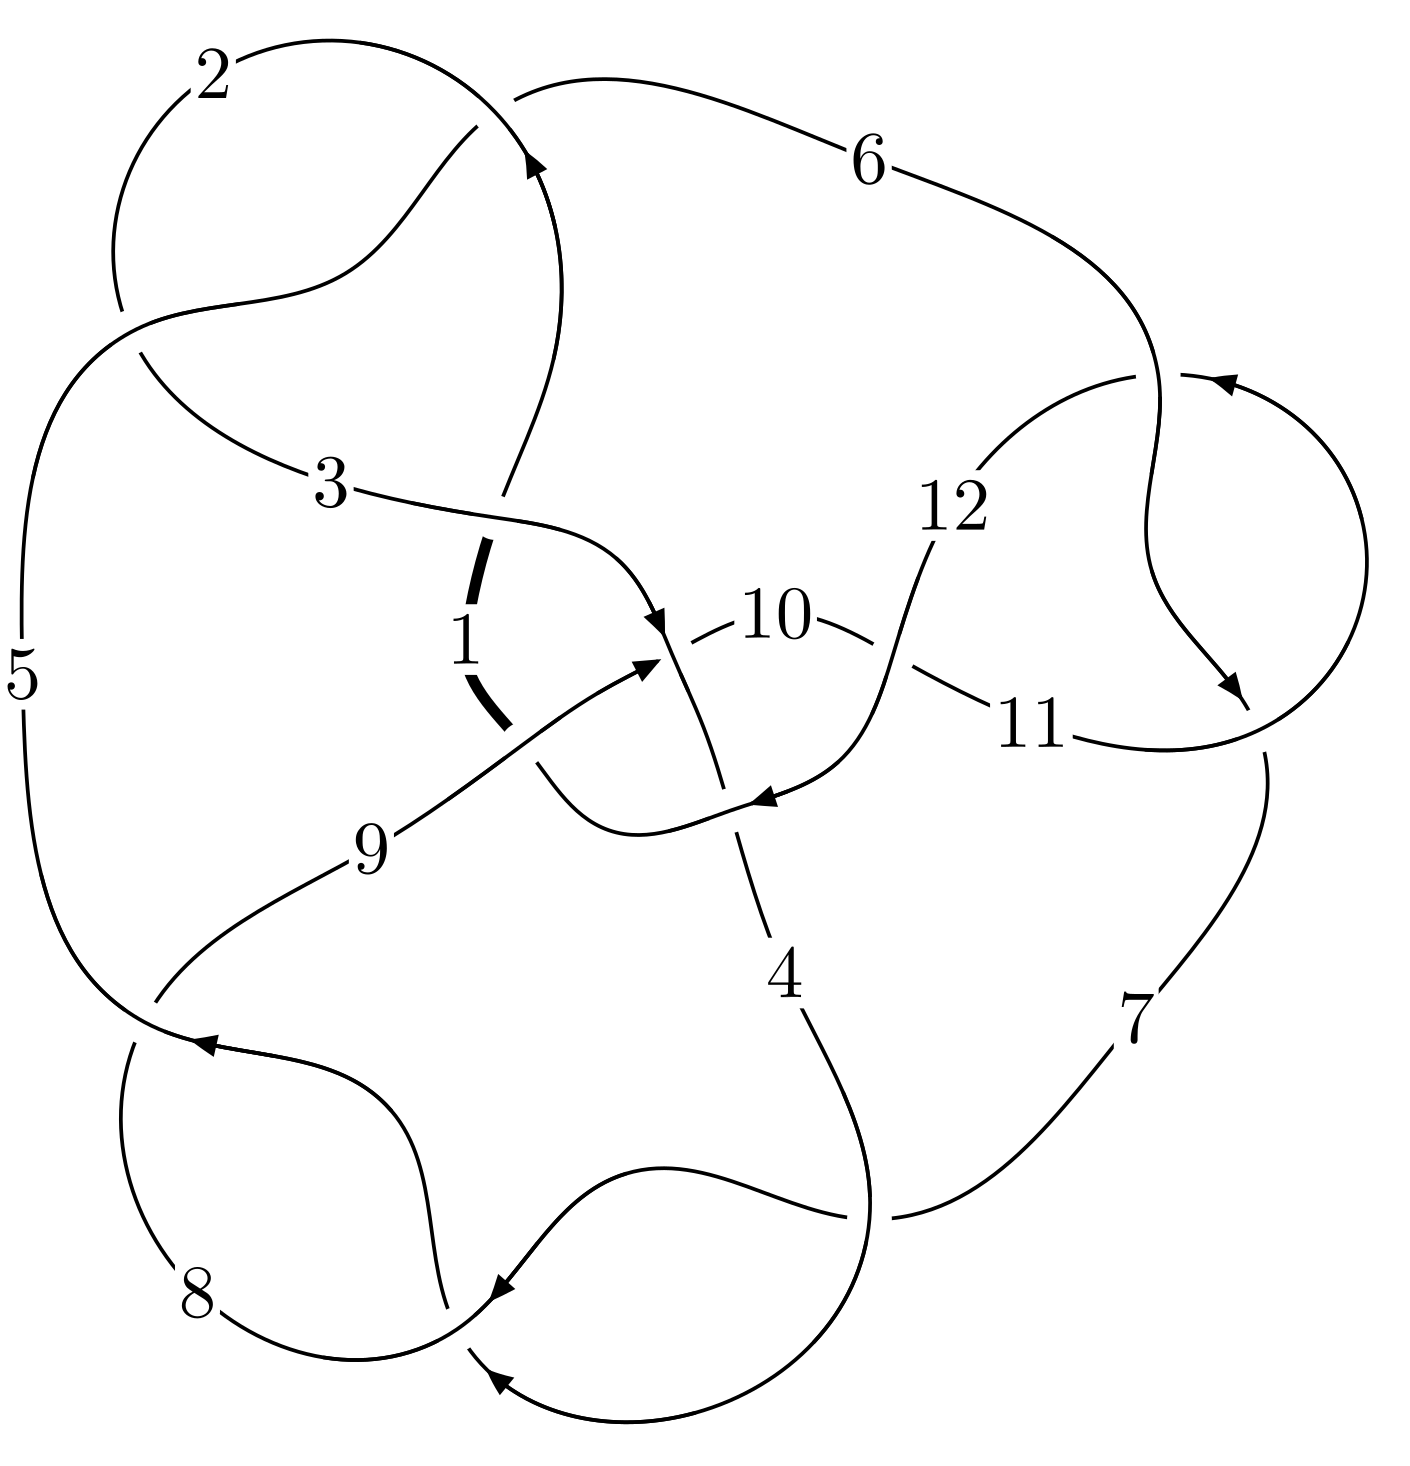
\includegraphics[width=112pt]{../../../GIT/diagram.site/Diagrams/png/2608_12n_0519.png}\\
\ \ \ A knot diagram\footnotemark}&
\allowdisplaybreaks
\textbf{Linearized knot diagam} \\
\cline{2-2}
 &
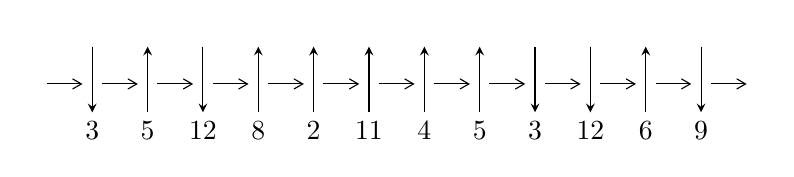
\begin{tikzpicture}[x=20pt, y=17pt]
	% nodes
	\node (C0) at (0, 0) {};
	\node (C1) at (1, 0) {};
	\node (C1U) at (1, +1) {};
	\node (C1D) at (1, -1) {3};

	\node (C2) at (2, 0) {};
	\node (C2U) at (2, +1) {};
	\node (C2D) at (2, -1) {5};

	\node (C3) at (3, 0) {};
	\node (C3U) at (3, +1) {};
	\node (C3D) at (3, -1) {12};

	\node (C4) at (4, 0) {};
	\node (C4U) at (4, +1) {};
	\node (C4D) at (4, -1) {8};

	\node (C5) at (5, 0) {};
	\node (C5U) at (5, +1) {};
	\node (C5D) at (5, -1) {2};

	\node (C6) at (6, 0) {};
	\node (C6U) at (6, +1) {};
	\node (C6D) at (6, -1) {11};

	\node (C7) at (7, 0) {};
	\node (C7U) at (7, +1) {};
	\node (C7D) at (7, -1) {4};

	\node (C8) at (8, 0) {};
	\node (C8U) at (8, +1) {};
	\node (C8D) at (8, -1) {5};

	\node (C9) at (9, 0) {};
	\node (C9U) at (9, +1) {};
	\node (C9D) at (9, -1) {3};

	\node (C10) at (10, 0) {};
	\node (C10U) at (10, +1) {};
	\node (C10D) at (10, -1) {12};

	\node (C11) at (11, 0) {};
	\node (C11U) at (11, +1) {};
	\node (C11D) at (11, -1) {6};

	\node (C12) at (12, 0) {};
	\node (C12U) at (12, +1) {};
	\node (C12D) at (12, -1) {9};
	\node (C13) at (13, 0) {};

	% arrows
	\draw[->,>={angle 60}]
	(C0) edge (C1) (C1) edge (C2) (C2) edge (C3) (C3) edge (C4) (C4) edge (C5) (C5) edge (C6) (C6) edge (C7) (C7) edge (C8) (C8) edge (C9) (C9) edge (C10) (C10) edge (C11) (C11) edge (C12) (C12) edge (C13) ;	\draw[->,>=stealth]
	(C1U) edge (C1D) (C2D) edge (C2U) (C3U) edge (C3D) (C4D) edge (C4U) (C5D) edge (C5U) (C6D) edge (C6U) (C7D) edge (C7U) (C8D) edge (C8U) (C9U) edge (C9D) (C10U) edge (C10D) (C11D) edge (C11U) (C12U) edge (C12D) ;
	\end{tikzpicture} \\
\hhline{~~} \\& 
\textbf{Solving Sequence} \\ \cline{2-2} 
 &
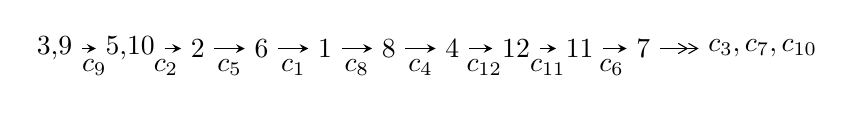
\begin{tikzpicture}[x=23pt, y=7pt]
	% node
	\node (A0) at (-1/8, 0) {3,9};
	\node (A1) at (17/16, 0) {5,10};
	\node (A2) at (17/8, 0) {2};
	\node (A3) at (25/8, 0) {6};
	\node (A4) at (33/8, 0) {1};
	\node (A5) at (41/8, 0) {8};
	\node (A6) at (49/8, 0) {4};
	\node (A7) at (57/8, 0) {12};
	\node (A8) at (65/8, 0) {11};
	\node (A9) at (73/8, 0) {7};
	\node (C1) at (1/2, -1) {$c_{9}$};
	\node (C2) at (13/8, -1) {$c_{2}$};
	\node (C3) at (21/8, -1) {$c_{5}$};
	\node (C4) at (29/8, -1) {$c_{1}$};
	\node (C5) at (37/8, -1) {$c_{8}$};
	\node (C6) at (45/8, -1) {$c_{4}$};
	\node (C7) at (53/8, -1) {$c_{12}$};
	\node (C8) at (61/8, -1) {$c_{11}$};
	\node (C9) at (69/8, -1) {$c_{6}$};
	\node (A10) at (11, 0) {$c_{3},c_{7},c_{10}$};

	% edge
	\draw[->,>=stealth]	
	(A0) edge (A1) (A1) edge (A2) (A2) edge (A3) (A3) edge (A4) (A4) edge (A5) (A5) edge (A6) (A6) edge (A7) (A7) edge (A8) (A8) edge (A9) ;
	\draw[->>,>={angle 60}]	
	(A9) edge (A10);
\end{tikzpicture} \\ 

\end{tabular} \\

\footnotetext{
The image of knot diagram is generated by the software ``\textbf{Draw programme}" developed by Andrew Bartholomew(\url{http://www.layer8.co.uk/maths/draw/index.htm\#Running-draw}), where we modified some parts for our purpose(\url{https://github.com/CATsTAILs/LinksPainter}).
}\phantom \\ \newline 
\centering \textbf{Ideals for irreducible components\footnotemark of $X_{\text{par}}$} 
 
\begin{align*}
I^u_{1}&=\langle 
58 u^9-249 u^8-444 u^7+2113 u^6+1475 u^5-7574 u^4+2612 u^3+2889 u^2+349 b-1335 u-353,\\
\phantom{I^u_{1}}&\phantom{= \langle  }-2528 u^9+8422 u^8+\cdots+1745 a-16349,\\
\phantom{I^u_{1}}&\phantom{= \langle  }u^{10}-4 u^9-3 u^8+29 u^7-14 u^6-89 u^5+163 u^4-109 u^3+17 u^2+13 u-5\rangle \\
I^u_{2}&=\langle 
-88 u^6+345 u^5-33 u^4-837 u^3-116 u^2+719 b+189 u+50,\\
\phantom{I^u_{2}}&\phantom{= \langle  }267 u^6-1202 u^5+909 u^4+1747 u^3+1169 u^2+5033 a-5010 u+649,\\
\phantom{I^u_{2}}&\phantom{= \langle  }u^7-5 u^6+6 u^5+4 u^4-7 u^3+2 u^2+5 u-7\rangle \\
I^u_{3}&=\langle 
u^3+b-3 u-2,\;u^3 a-3 u^3+a^2-3 a u- a+10 u,\;u^4+u^3-3 u^2-3 u-1\rangle \\
I^u_{4}&=\langle 
u^3+2 u^2+b- u-2,\;u^3 a+2 u^2 a-3 u^3+a^2- a u-8 u^2-3 a+10,\;u^4+3 u^3+u^2-3 u-1\rangle \\
\\
\end{align*}
\raggedright * 4 irreducible components of $\dim_{\mathbb{C}}=0$, with total 33 representations.\\
\footnotetext{All coefficients of polynomials are rational numbers. But the coefficients are sometimes approximated in decimal forms when there is not enough margin.}
\newpage
\renewcommand{\arraystretch}{1}
\centering \section*{I. $I^u_{1}= \langle 58 u^9-249 u^8+\cdots+349 b-353,\;-2528 u^9+8422 u^8+\cdots+1745 a-16349,\;u^{10}-4 u^9+\cdots+13 u-5 \rangle$}
\flushleft \textbf{(i) Arc colorings}\\
\begin{tabular}{m{7pt} m{180pt} m{7pt} m{180pt} }
\flushright $a_{3}=$&$\begin{pmatrix}0\\u\end{pmatrix}$ \\
\flushright $a_{9}=$&$\begin{pmatrix}1\\0\end{pmatrix}$ \\
\flushright $a_{5}=$&$\begin{pmatrix}1.44871 u^{9}-4.82636 u^{8}+\cdots-13.0281 u+9.36905\\-0.166189 u^{9}+0.713467 u^{8}+\cdots+3.82521 u+1.01146\end{pmatrix}$ \\
\flushright $a_{10}=$&$\begin{pmatrix}1\\u^2\end{pmatrix}$ \\
\flushright $a_{2}=$&$\begin{pmatrix}0.0710602 u^{9}-0.436103 u^{8}+\cdots-1.40802 u+1.50544\\-0.260745 u^{9}+0.446991 u^{8}+\cdots+1.43266 u+0.742120\end{pmatrix}$ \\
\flushright $a_{6}=$&$\begin{pmatrix}1.07736 u^{9}-3.41834 u^{8}+\cdots-8.31519 u+5.85673\\0.00286533 u^{9}+0.280802 u^{8}+\cdots+1.95129 u-0.931232\end{pmatrix}$ \\
\flushright $a_{1}=$&$\begin{pmatrix}0.0710602 u^{9}-0.436103 u^{8}+\cdots-1.40802 u+1.50544\\0.229226 u^{9}-0.535817 u^{8}+\cdots-0.896848 u+1.50143\end{pmatrix}$ \\
\flushright $a_{8}=$&$\begin{pmatrix}-0.148424 u^{9}+0.854441 u^{8}+\cdots+1.72321 u-1.36218\\1.39542 u^{9}-4.24928 u^{8}+\cdots-12.7221 u+5.48997\end{pmatrix}$ \\
\flushright $a_{4}=$&$\begin{pmatrix}-0.0108883 u^{9}-0.667049 u^{8}+\cdots-2.61490 u-0.0613181\\-0.710602 u^{9}+0.361032 u^{8}+\cdots+1.08023 u-0.0544413\end{pmatrix}$ \\
\flushright $a_{12}=$&$\begin{pmatrix}0.300287 u^{9}-0.971920 u^{8}+\cdots-2.30487 u+3.00688\\0.229226 u^{9}-0.535817 u^{8}+\cdots-0.896848 u+1.50143\end{pmatrix}$ \\
\flushright $a_{11}=$&$\begin{pmatrix}-0.699713 u^{9}+1.02808 u^{8}+\cdots+2.69513 u+1.00688\\-1.77077 u^{9}+3.46418 u^{8}+\cdots+9.10315 u-3.49857\end{pmatrix}$ \\
\flushright $a_{7}=$&$\begin{pmatrix}1.40802 u^{9}-3.21375 u^{8}+\cdots-6.53639 u+1.19255\\1.23496 u^{9}-2.97421 u^{8}+\cdots-6.99427 u+1.63897\end{pmatrix}$\\&\end{tabular}
\flushleft \textbf{(ii) Obstruction class $= -1$}\\~\\
\flushleft \textbf{(iii) Cusp Shapes $= \frac{150}{349} u^9+\frac{391}{349} u^8-\frac{3146}{349} u^7-\frac{2093}{349} u^6+\frac{18942}{349} u^5-\frac{417}{349} u^4-\frac{51937}{349} u^3+\frac{49159}{349} u^2-\frac{6389}{349} u-\frac{6172}{349}$}\\~\\
\newpage\renewcommand{\arraystretch}{1}
\flushleft \textbf{(iv) u-Polynomials at the component}\newline \\
\begin{tabular}{m{50pt}|m{274pt}}
Crossings & \hspace{64pt}u-Polynomials at each crossing \\
\hline $$\begin{aligned}c_{1},c_{10}\end{aligned}$$&$\begin{aligned}
&u^{10}+6 u^9+\cdots+4 u+1
\end{aligned}$\\
\hline $$\begin{aligned}c_{2},c_{5},c_{6}\\c_{11}\end{aligned}$$&$\begin{aligned}
&u^{10}+3 u^8-6 u^7+4 u^6-17 u^5+4 u^4-11 u^3+4 u^2-2 u+1
\end{aligned}$\\
\hline $$\begin{aligned}c_{3},c_{12}\end{aligned}$$&$\begin{aligned}
&u^{10}+2 u^9+29 u^7+73 u^6+119 u^5+136 u^4+94 u^3+32 u^2+2 u-1
\end{aligned}$\\
\hline $$\begin{aligned}c_{4},c_{7},c_{8}\end{aligned}$$&$\begin{aligned}
&u^{10}-7 u^9+\cdots+8 u-8
\end{aligned}$\\
\hline $$\begin{aligned}c_{9}\end{aligned}$$&$\begin{aligned}
&u^{10}+4 u^9+\cdots-13 u-5
\end{aligned}$\\
\hline
\end{tabular}\\~\\
\newpage\renewcommand{\arraystretch}{1}
\flushleft \textbf{(v) Riley Polynomials at the component}\newline \\
\begin{tabular}{m{50pt}|m{274pt}}
Crossings & \hspace{64pt}Riley Polynomials at each crossing \\
\hline $$\begin{aligned}c_{1},c_{10}\end{aligned}$$&$\begin{aligned}
&y^{10}-2 y^9+\cdots-56 y+1
\end{aligned}$\\
\hline $$\begin{aligned}c_{2},c_{5},c_{6}\\c_{11}\end{aligned}$$&$\begin{aligned}
&y^{10}+6 y^9+\cdots+4 y+1
\end{aligned}$\\
\hline $$\begin{aligned}c_{3},c_{12}\end{aligned}$$&$\begin{aligned}
&y^{10}-4 y^9+\cdots-68 y+1
\end{aligned}$\\
\hline $$\begin{aligned}c_{4},c_{7},c_{8}\end{aligned}$$&$\begin{aligned}
&y^{10}-19 y^9+\cdots-352 y+64
\end{aligned}$\\
\hline $$\begin{aligned}c_{9}\end{aligned}$$&$\begin{aligned}
&y^{10}-22 y^9+\cdots-339 y+25
\end{aligned}$\\
\hline
\end{tabular}\\~\\
\newpage\flushleft \textbf{(vi) Complex Volumes and Cusp Shapes}
$$\begin{array}{c|c|c}  
\text{Solutions to }I^u_{1}& \I (\text{vol} + \sqrt{-1}CS) & \text{Cusp shape}\\
 \hline 
\begin{aligned}
u &= \phantom{-}0.710716 + 0.441346 I \\
a &= \phantom{-}0.304205 + 0.895172 I \\
b &= -1.53379 - 0.01592 I\end{aligned}
 & \phantom{-}5.27109 - 1.67493 I & \phantom{-}4.82619 + 2.79664 I \\ \hline\begin{aligned}
u &= \phantom{-}0.710716 - 0.441346 I \\
a &= \phantom{-}0.304205 - 0.895172 I \\
b &= -1.53379 + 0.01592 I\end{aligned}
 & \phantom{-}5.27109 + 1.67493 I & \phantom{-}4.82619 - 2.79664 I \\ \hline\begin{aligned}
u &= \phantom{-}0.610288 + 0.265211 I \\
a &= -0.344245 - 0.794267 I \\
b &= \phantom{-}0.382201 - 0.301034 I\end{aligned}
 & -1.12041 - 1.07831 I & -3.35767 + 4.98904 I \\ \hline\begin{aligned}
u &= \phantom{-}0.610288 - 0.265211 I \\
a &= -0.344245 + 0.794267 I \\
b &= \phantom{-}0.382201 + 0.301034 I\end{aligned}
 & -1.12041 + 1.07831 I & -3.35767 - 4.98904 I \\ \hline\begin{aligned}
u &= -0.348971\phantom{ +0.000000I} \\
a &= -1.18540\phantom{ +0.000000I} \\
b &= -0.681296\phantom{ +0.000000I}\end{aligned}
 & \phantom{-}0.925697\phantom{ +0.000000I} & \phantom{-}11.8780\phantom{ +0.000000I} \\ \hline\begin{aligned}
u &= \phantom{-}1.85552\phantom{ +0.000000I} \\
a &= \phantom{-}0.910166\phantom{ +0.000000I} \\
b &= \phantom{-}2.25830\phantom{ +0.000000I}\end{aligned}
 & \phantom{-}1.90296\phantom{ +0.000000I} & \phantom{-}4.31530\phantom{ +0.000000I} \\ \hline\begin{aligned}
u &= \phantom{-}2.12102 + 0.16943 I \\
a &= -0.392434 + 0.798856 I \\
b &= -2.19435 + 0.73311 I\end{aligned}
 & \phantom{-}15.2945 - 10.5947 I & \phantom{-}2.32893 + 3.81440 I \\ \hline\begin{aligned}
u &= \phantom{-}2.12102 - 0.16943 I \\
a &= -0.392434 - 0.798856 I \\
b &= -2.19435 - 0.73311 I\end{aligned}
 & \phantom{-}15.2945 + 10.5947 I & \phantom{-}2.32893 - 3.81440 I \\ \hline\begin{aligned}
u &= -2.19529 + 0.82711 I \\
a &= \phantom{-}0.170094 - 0.566049 I \\
b &= -0.942562 - 0.925156 I\end{aligned}
 & -8.52247 + 3.39717 I & \phantom{-}0.10586 - 5.05917 I \\ \hline\begin{aligned}
u &= -2.19529 - 0.82711 I \\
a &= \phantom{-}0.170094 + 0.566049 I \\
b &= -0.942562 + 0.925156 I\end{aligned}
 & -8.52247 - 3.39717 I & \phantom{-}0.10586 + 5.05917 I\\
 \hline 
 \end{array}$$\newpage\newpage\renewcommand{\arraystretch}{1}
\centering \section*{II. $I^u_{2}= \langle -88 u^6+345 u^5+\cdots+719 b+50,\;267 u^6-1202 u^5+\cdots+5033 a+649,\;u^7-5 u^6+6 u^5+4 u^4-7 u^3+2 u^2+5 u-7 \rangle$}
\flushleft \textbf{(i) Arc colorings}\\
\begin{tabular}{m{7pt} m{180pt} m{7pt} m{180pt} }
\flushright $a_{3}=$&$\begin{pmatrix}0\\u\end{pmatrix}$ \\
\flushright $a_{9}=$&$\begin{pmatrix}1\\0\end{pmatrix}$ \\
\flushright $a_{5}=$&$\begin{pmatrix}-0.0530499 u^{6}+0.238824 u^{5}+\cdots+0.995430 u-0.128949\\0.122392 u^{6}-0.479833 u^{5}+\cdots-0.262865 u-0.0695410\end{pmatrix}$ \\
\flushright $a_{10}=$&$\begin{pmatrix}1\\u^2\end{pmatrix}$ \\
\flushright $a_{2}=$&$\begin{pmatrix}0.0202662 u^{6}-0.271011 u^{5}+\cdots+0.271409 u+0.397576\\-0.0792768 u^{6}+0.413074 u^{5}+\cdots+1.40890 u-1.11405\end{pmatrix}$ \\
\flushright $a_{6}=$&$\begin{pmatrix}-0.0103318 u^{6}+0.0989470 u^{5}+\cdots-0.412875 u+0.914961\\-0.0152990 u^{6}+0.184979 u^{5}+\cdots+0.657858 u+0.258693\end{pmatrix}$ \\
\flushright $a_{1}=$&$\begin{pmatrix}0.0202662 u^{6}-0.271011 u^{5}+\cdots+0.271409 u+0.397576\\-0.00973574 u^{6}+0.208623 u^{5}+\cdots+0.418637 u+0.0737135\end{pmatrix}$ \\
\flushright $a_{8}=$&$\begin{pmatrix}0.159150 u^{6}-0.716471 u^{5}+\cdots-0.986290 u+1.38685\\-0.0695410 u^{6}+0.204451 u^{5}+\cdots+0.990264 u+0.812239\end{pmatrix}$ \\
\flushright $a_{4}=$&$\begin{pmatrix}0.00993443 u^{6}-0.172064 u^{5}+\cdots-0.141466 u+0.312537\\-0.122392 u^{6}+0.479833 u^{5}+\cdots+1.26287 u+0.0695410\end{pmatrix}$ \\
\flushright $a_{12}=$&$\begin{pmatrix}0.0105305 u^{6}-0.0623882 u^{5}+\cdots+0.690046 u+0.471289\\-0.00973574 u^{6}+0.208623 u^{5}+\cdots+0.418637 u+0.0737135\end{pmatrix}$ \\
\flushright $a_{11}=$&$\begin{pmatrix}-0.132327 u^{6}+0.651897 u^{5}+\cdots+0.404331 u+0.757004\\-0.00973574 u^{6}+0.208623 u^{5}+\cdots+0.418637 u-0.926287\end{pmatrix}$ \\
\flushright $a_{7}=$&$\begin{pmatrix}0.0431154 u^{6}-0.0667594 u^{5}+\cdots-0.853964 u-0.183588\\0.132128 u^{6}-0.688456 u^{5}+\cdots-0.681502 u+0.856745\end{pmatrix}$\\&\end{tabular}
\flushleft \textbf{(ii) Obstruction class $= 1$}\\~\\
\flushleft \textbf{(iii) Cusp Shapes $= -\frac{334}{719} u^6+\frac{1816}{719} u^5-\frac{2462}{719} u^4-\frac{742}{719} u^3+\frac{148}{719} u^2+\frac{2139}{719} u-\frac{39}{719}$}\\~\\
\newpage\renewcommand{\arraystretch}{1}
\flushleft \textbf{(iv) u-Polynomials at the component}\newline \\
\begin{tabular}{m{50pt}|m{274pt}}
Crossings & \hspace{64pt}u-Polynomials at each crossing \\
\hline $$\begin{aligned}c_{1},c_{10}\end{aligned}$$&$\begin{aligned}
&u^7-7 u^6+22 u^5-41 u^4+48 u^3-33 u^2+10 u+1
\end{aligned}$\\
\hline $$\begin{aligned}c_{2},c_{6}\end{aligned}$$&$\begin{aligned}
&u^7+u^6+4 u^5+3 u^4+6 u^3+3 u^2+4 u+1
\end{aligned}$\\
\hline $$\begin{aligned}c_{3},c_{12}\end{aligned}$$&$\begin{aligned}
&u^7- u^6+u^5- u^4- u^3+u^2+1
\end{aligned}$\\
\hline $$\begin{aligned}c_{4}\end{aligned}$$&$\begin{aligned}
&u^7- u^6-3 u^5+u^4+5 u^3- u^2-2 u+1
\end{aligned}$\\
\hline $$\begin{aligned}c_{5},c_{11}\end{aligned}$$&$\begin{aligned}
&u^7- u^6+4 u^5-3 u^4+6 u^3-3 u^2+4 u-1
\end{aligned}$\\
\hline $$\begin{aligned}c_{7},c_{8}\end{aligned}$$&$\begin{aligned}
&u^7+u^6-3 u^5- u^4+5 u^3+u^2-2 u-1
\end{aligned}$\\
\hline $$\begin{aligned}c_{9}\end{aligned}$$&$\begin{aligned}
&u^7-5 u^6+6 u^5+4 u^4-7 u^3+2 u^2+5 u-7
\end{aligned}$\\
\hline
\end{tabular}\\~\\
\newpage\renewcommand{\arraystretch}{1}
\flushleft \textbf{(v) Riley Polynomials at the component}\newline \\
\begin{tabular}{m{50pt}|m{274pt}}
Crossings & \hspace{64pt}Riley Polynomials at each crossing \\
\hline $$\begin{aligned}c_{1},c_{10}\end{aligned}$$&$\begin{aligned}
&y^7-5 y^6+6 y^5-11 y^4+52 y^3-47 y^2+166 y-1
\end{aligned}$\\
\hline $$\begin{aligned}c_{2},c_{5},c_{6}\\c_{11}\end{aligned}$$&$\begin{aligned}
&y^7+7 y^6+22 y^5+41 y^4+48 y^3+33 y^2+10 y-1
\end{aligned}$\\
\hline $$\begin{aligned}c_{3},c_{12}\end{aligned}$$&$\begin{aligned}
&y^7+y^6-3 y^5- y^4+5 y^3+y^2-2 y-1
\end{aligned}$\\
\hline $$\begin{aligned}c_{4},c_{7},c_{8}\end{aligned}$$&$\begin{aligned}
&y^7-7 y^6+21 y^5-37 y^4+41 y^3-23 y^2+6 y-1
\end{aligned}$\\
\hline $$\begin{aligned}c_{9}\end{aligned}$$&$\begin{aligned}
&y^7-13 y^6+62 y^5-70 y^4+23 y^3-18 y^2+53 y-49
\end{aligned}$\\
\hline
\end{tabular}\\~\\
\newpage\flushleft \textbf{(vi) Complex Volumes and Cusp Shapes}
$$\begin{array}{c|c|c}  
\text{Solutions to }I^u_{2}& \I (\text{vol} + \sqrt{-1}CS) & \text{Cusp shape}\\
 \hline 
\begin{aligned}
u &= -0.942087 + 0.385621 I \\
a &= -0.961712 + 0.696018 I \\
b &= -0.470376 + 0.273309 I\end{aligned}
 & \phantom{-}0.08815 - 5.09905 I & -0.97794 + 6.62021 I \\ \hline\begin{aligned}
u &= -0.942087 - 0.385621 I \\
a &= -0.961712 - 0.696018 I \\
b &= -0.470376 - 0.273309 I\end{aligned}
 & \phantom{-}0.08815 + 5.09905 I & -0.97794 - 6.62021 I \\ \hline\begin{aligned}
u &= \phantom{-}0.401929 + 0.876655 I \\
a &= \phantom{-}0.865092 + 0.818149 I \\
b &= -1.53400 - 0.17432 I\end{aligned}
 & \phantom{-}4.42380 - 3.02243 I & \phantom{-}3.79268 + 4.58771 I \\ \hline\begin{aligned}
u &= \phantom{-}0.401929 - 0.876655 I \\
a &= \phantom{-}0.865092 - 0.818149 I \\
b &= -1.53400 + 0.17432 I\end{aligned}
 & \phantom{-}4.42380 + 3.02243 I & \phantom{-}3.79268 - 4.58771 I \\ \hline\begin{aligned}
u &= \phantom{-}1.08372\phantom{ +0.000000I} \\
a &= \phantom{-}0.257183\phantom{ +0.000000I} \\
b &= \phantom{-}0.861033\phantom{ +0.000000I}\end{aligned}
 & -0.272703\phantom{ +0.000000I} & \phantom{-}0.397920\phantom{ +0.000000I} \\ \hline\begin{aligned}
u &= \phantom{-}2.49830 + 0.67865 I \\
a &= -0.103399 - 0.517020 I \\
b &= \phantom{-}1.073860 - 0.702292 I\end{aligned}
 & -9.31040 - 2.64371 I & -5.01371 + 0.82640 I \\ \hline\begin{aligned}
u &= \phantom{-}2.49830 - 0.67865 I \\
a &= -0.103399 + 0.517020 I \\
b &= \phantom{-}1.073860 + 0.702292 I\end{aligned}
 & -9.31040 + 2.64371 I & -5.01371 - 0.82640 I\\
 \hline 
 \end{array}$$\newpage\newpage\renewcommand{\arraystretch}{1}
\centering \section*{III. $I^u_{3}= \langle u^3+b-3 u-2,\;u^3 a-3 u^3+a^2-3 a u- a+10 u,\;u^4+u^3-3 u^2-3 u-1 \rangle$}
\flushleft \textbf{(i) Arc colorings}\\
\begin{tabular}{m{7pt} m{180pt} m{7pt} m{180pt} }
\flushright $a_{3}=$&$\begin{pmatrix}0\\u\end{pmatrix}$ \\
\flushright $a_{9}=$&$\begin{pmatrix}1\\0\end{pmatrix}$ \\
\flushright $a_{5}=$&$\begin{pmatrix}a\\- u^3+3 u+2\end{pmatrix}$ \\
\flushright $a_{10}=$&$\begin{pmatrix}1\\u^2\end{pmatrix}$ \\
\flushright $a_{2}=$&$\begin{pmatrix}- u^3 a+3 u^3+2 a u+u^2+a-9 u-3\\- u^3 a+a u+a+u\end{pmatrix}$ \\
\flushright $a_{6}=$&$\begin{pmatrix}2 u^2 a+u^3-3 a u-2 u^2- a- u+1\\-3 u^3 a+2 u^2 a+2 u^3+5 a u-2 u^2+2 a-4 u\end{pmatrix}$ \\
\flushright $a_{1}=$&$\begin{pmatrix}- u^3 a+3 u^3+2 a u+u^2+a-9 u-3\\u^3 a- u^2 a-2 u^3- a u+4 u+2\end{pmatrix}$ \\
\flushright $a_{8}=$&$\begin{pmatrix}- u^3 a+3 a u+2 a+1\\-2 u^3+u^2+5 u+2\end{pmatrix}$ \\
\flushright $a_{4}=$&$\begin{pmatrix}2 u^3 a- u^2 a+u^3-5 a u- a-3 u-2\\3 u^3-4 u^2-4 u\end{pmatrix}$ \\
\flushright $a_{12}=$&$\begin{pmatrix}- u^2 a+u^3+a u+u^2+a-5 u-1\\u^3 a- u^2 a-2 u^3- a u+4 u+2\end{pmatrix}$ \\
\flushright $a_{11}=$&$\begin{pmatrix}-3 u^3 a+u^2 a- u^3+5 a u-3 u^2+2 a+5 u+7\\-3 u^3 a+u^2 a-2 u^3+5 a u+u^2+2 a+4 u+1\end{pmatrix}$ \\
\flushright $a_{7}=$&$\begin{pmatrix}-2 u^3 a+4 u^2 a-2 u^3+a u+u^2-2 a+5 u+1\\-7 u^3+10 u^2+5 u+1\end{pmatrix}$\\&\end{tabular}
\flushleft \textbf{(ii) Obstruction class $= -1$}\\~\\
\flushleft \textbf{(iii) Cusp Shapes $= -2 u^3- u^2+6 u+5$}\\~\\
\newpage\renewcommand{\arraystretch}{1}
\flushleft \textbf{(iv) u-Polynomials at the component}\newline \\
\begin{tabular}{m{50pt}|m{274pt}}
Crossings & \hspace{64pt}u-Polynomials at each crossing \\
\hline $$\begin{aligned}c_{1},c_{10}\end{aligned}$$&$\begin{aligned}
&u^8- u^7+16 u^6+69 u^5+299 u^4+497 u^3+868 u^2+535 u+841
\end{aligned}$\\
\hline $$\begin{aligned}c_{2},c_{5},c_{6}\\c_{11}\end{aligned}$$&$\begin{aligned}
&u^8+3 u^7+4 u^6+7 u^5+21 u^4+15 u^3+20 u^2+25 u+29
\end{aligned}$\\
\hline $$\begin{aligned}c_{3},c_{12}\end{aligned}$$&$\begin{aligned}
&u^8-6 u^7+38 u^6-114 u^5+133 u^4-82 u^3+227 u^2-449 u+431
\end{aligned}$\\
\hline $$\begin{aligned}c_{4},c_{7},c_{8}\end{aligned}$$&$\begin{aligned}
&(u^4+6 u^3+12 u^2+11 u+5)^2
\end{aligned}$\\
\hline $$\begin{aligned}c_{9}\end{aligned}$$&$\begin{aligned}
&(u^4- u^3-3 u^2+3 u-1)^2
\end{aligned}$\\
\hline
\end{tabular}\\~\\
\newpage\renewcommand{\arraystretch}{1}
\flushleft \textbf{(v) Riley Polynomials at the component}\newline \\
\begin{tabular}{m{50pt}|m{274pt}}
Crossings & \hspace{64pt}Riley Polynomials at each crossing \\
\hline $$\begin{aligned}c_{1},c_{10}\end{aligned}$$&$\begin{aligned}
&y^8+31 y^7+\cdots+1173751 y+707281
\end{aligned}$\\
\hline $$\begin{aligned}c_{2},c_{5},c_{6}\\c_{11}\end{aligned}$$&$\begin{aligned}
&y^8- y^7+16 y^6+69 y^5+299 y^4+497 y^3+868 y^2+535 y+841
\end{aligned}$\\
\hline $$\begin{aligned}c_{3},c_{12}\end{aligned}$$&$\begin{aligned}
&y^8+40 y^7+\cdots-5927 y+185761
\end{aligned}$\\
\hline $$\begin{aligned}c_{4},c_{7},c_{8}\end{aligned}$$&$\begin{aligned}
&(y^4-12 y^3+22 y^2- y+25)^2
\end{aligned}$\\
\hline $$\begin{aligned}c_{9}\end{aligned}$$&$\begin{aligned}
&(y^4-7 y^3+13 y^2-3 y+1)^2
\end{aligned}$\\
\hline
\end{tabular}\\~\\
\newpage\flushleft \textbf{(vi) Complex Volumes and Cusp Shapes}
$$\begin{array}{c|c|c}  
\text{Solutions to }I^u_{3}& \I (\text{vol} + \sqrt{-1}CS) & \text{Cusp shape}\\
 \hline 
\begin{aligned}
u &= -0.447135 + 0.308371 I \\
a &= \phantom{-}2.01612 - 0.24150 I \\
b &= \phantom{-}0.620433 + 0.769480 I\end{aligned}
 & \phantom{-}0.96275 - 3.58171 I & \phantom{-}2.13603 + 1.81473 I \\ \hline\begin{aligned}
u &= -0.447135 + 0.308371 I \\
a &= -2.39569 + 1.01098 I \\
b &= \phantom{-}0.620433 + 0.769480 I\end{aligned}
 & \phantom{-}0.96275 - 3.58171 I & \phantom{-}2.13603 + 1.81473 I \\ \hline\begin{aligned}
u &= -0.447135 - 0.308371 I \\
a &= \phantom{-}2.01612 + 0.24150 I \\
b &= \phantom{-}0.620433 - 0.769480 I\end{aligned}
 & \phantom{-}0.96275 + 3.58171 I & \phantom{-}2.13603 - 1.81473 I \\ \hline\begin{aligned}
u &= -0.447135 - 0.308371 I \\
a &= -2.39569 - 1.01098 I \\
b &= \phantom{-}0.620433 - 0.769480 I\end{aligned}
 & \phantom{-}0.96275 + 3.58171 I & \phantom{-}2.13603 - 1.81473 I \\ \hline\begin{aligned}
u &= \phantom{-}1.78897\phantom{ +0.000000I} \\
a &= \phantom{-}0.320723 + 0.781310 I \\
b &= \phantom{-}1.64145\phantom{ +0.000000I}\end{aligned}
 & -7.09598\phantom{ +0.000000I} & \phantom{-}1.08250\phantom{ +0.000000I} \\ \hline\begin{aligned}
u &= \phantom{-}1.78897\phantom{ +0.000000I} \\
a &= \phantom{-}0.320723 - 0.781310 I \\
b &= \phantom{-}1.64145\phantom{ +0.000000I}\end{aligned}
 & -7.09598\phantom{ +0.000000I} & \phantom{-}1.08250\phantom{ +0.000000I} \\ \hline\begin{aligned}
u &= -1.89470\phantom{ +0.000000I} \\
a &= \phantom{-}1.058840 + 0.580699 I \\
b &= \phantom{-}3.11769\phantom{ +0.000000I}\end{aligned}
 & \phantom{-}18.3299\phantom{ +0.000000I} & \phantom{-}3.64550\phantom{ +0.000000I} \\ \hline\begin{aligned}
u &= -1.89470\phantom{ +0.000000I} \\
a &= \phantom{-}1.058840 - 0.580699 I \\
b &= \phantom{-}3.11769\phantom{ +0.000000I}\end{aligned}
 & \phantom{-}18.3299\phantom{ +0.000000I} & \phantom{-}3.64550\phantom{ +0.000000I}\\
 \hline 
 \end{array}$$\newpage\newpage\renewcommand{\arraystretch}{1}
\centering \section*{IV. $I^u_{4}= \langle u^3+2 u^2+b- u-2,\;u^3 a+2 u^2 a-3 u^3+a^2- a u-8 u^2-3 a+10,\;u^4+3 u^3+u^2-3 u-1 \rangle$}
\flushleft \textbf{(i) Arc colorings}\\
\begin{tabular}{m{7pt} m{180pt} m{7pt} m{180pt} }
\flushright $a_{3}=$&$\begin{pmatrix}0\\u\end{pmatrix}$ \\
\flushright $a_{9}=$&$\begin{pmatrix}1\\0\end{pmatrix}$ \\
\flushright $a_{5}=$&$\begin{pmatrix}a\\- u^3-2 u^2+u+2\end{pmatrix}$ \\
\flushright $a_{10}=$&$\begin{pmatrix}1\\u^2\end{pmatrix}$ \\
\flushright $a_{2}=$&$\begin{pmatrix}- u^3 a-2 u^2 a+u^3+3 u^2+a+u-3\\- u^3 a-2 u^2 a+a u+a+u\end{pmatrix}$ \\
\flushright $a_{6}=$&$\begin{pmatrix}u^3+a u+2 u^2+a- u-3\\u^3 a- a u\end{pmatrix}$ \\
\flushright $a_{1}=$&$\begin{pmatrix}- u^3 a-2 u^2 a+u^3+3 u^2+a+u-3\\u^3 a+u^2 a- a u\end{pmatrix}$ \\
\flushright $a_{8}=$&$\begin{pmatrix}- u^3 a-2 u^2 a+a u+2 a+1\\- u^2- u+2\end{pmatrix}$ \\
\flushright $a_{4}=$&$\begin{pmatrix}u^2 a+u^3+a u+2 u^2- a- u-2\\u^3+2 u^2-2\end{pmatrix}$ \\
\flushright $a_{12}=$&$\begin{pmatrix}- u^2 a+u^3- a u+3 u^2+a+u-3\\u^3 a+u^2 a- a u\end{pmatrix}$ \\
\flushright $a_{11}=$&$\begin{pmatrix}u^3 a+u^2 a+u^3- a u+3 u^2+u-3\\u^3 a+u^2 a- a u+u^2-1\end{pmatrix}$ \\
\flushright $a_{7}=$&$\begin{pmatrix}a u+u^2+u-1\\u^3+2 u^2- u-1\end{pmatrix}$\\&\end{tabular}
\flushleft \textbf{(ii) Obstruction class $= 1$}\\~\\
\flushleft \textbf{(iii) Cusp Shapes $= -2 u^3-3 u^2+2 u+5$}\\~\\
\newpage\renewcommand{\arraystretch}{1}
\flushleft \textbf{(iv) u-Polynomials at the component}\newline \\
\begin{tabular}{m{50pt}|m{274pt}}
Crossings & \hspace{64pt}u-Polynomials at each crossing \\
\hline $$\begin{aligned}c_{1},c_{10}\end{aligned}$$&$\begin{aligned}
&u^8-7 u^7+20 u^6-33 u^5+39 u^4-33 u^3+20 u^2-7 u+1
\end{aligned}$\\
\hline $$\begin{aligned}c_{2},c_{6}\end{aligned}$$&$\begin{aligned}
&u^8+u^7+4 u^6+3 u^5+5 u^4+3 u^3+4 u^2+u+1
\end{aligned}$\\
\hline $$\begin{aligned}c_{3},c_{12}\end{aligned}$$&$\begin{aligned}
&u^8+4 u^7+6 u^6+4 u^5- u^4-4 u^3- u^2+u+1
\end{aligned}$\\
\hline $$\begin{aligned}c_{4}\end{aligned}$$&$\begin{aligned}
&(u^4-2 u^2+u+1)^2
\end{aligned}$\\
\hline $$\begin{aligned}c_{5},c_{11}\end{aligned}$$&$\begin{aligned}
&u^8- u^7+4 u^6-3 u^5+5 u^4-3 u^3+4 u^2- u+1
\end{aligned}$\\
\hline $$\begin{aligned}c_{7},c_{8}\end{aligned}$$&$\begin{aligned}
&(u^4-2 u^2- u+1)^2
\end{aligned}$\\
\hline $$\begin{aligned}c_{9}\end{aligned}$$&$\begin{aligned}
&(u^4+3 u^3+u^2-3 u-1)^2
\end{aligned}$\\
\hline
\end{tabular}\\~\\
\newpage\renewcommand{\arraystretch}{1}
\flushleft \textbf{(v) Riley Polynomials at the component}\newline \\
\begin{tabular}{m{50pt}|m{274pt}}
Crossings & \hspace{64pt}Riley Polynomials at each crossing \\
\hline $$\begin{aligned}c_{1},c_{10}\end{aligned}$$&$\begin{aligned}
&y^8-9 y^7+16 y^6+49 y^5+47 y^4+49 y^3+16 y^2-9 y+1
\end{aligned}$\\
\hline $$\begin{aligned}c_{2},c_{5},c_{6}\\c_{11}\end{aligned}$$&$\begin{aligned}
&y^8+7 y^7+20 y^6+33 y^5+39 y^4+33 y^3+20 y^2+7 y+1
\end{aligned}$\\
\hline $$\begin{aligned}c_{3},c_{12}\end{aligned}$$&$\begin{aligned}
&y^8-4 y^7+2 y^6+2 y^5+15 y^4-10 y^3+7 y^2-3 y+1
\end{aligned}$\\
\hline $$\begin{aligned}c_{4},c_{7},c_{8}\end{aligned}$$&$\begin{aligned}
&(y^4-4 y^3+6 y^2-5 y+1)^2
\end{aligned}$\\
\hline $$\begin{aligned}c_{9}\end{aligned}$$&$\begin{aligned}
&(y^4-7 y^3+17 y^2-11 y+1)^2
\end{aligned}$\\
\hline
\end{tabular}\\~\\
\newpage\flushleft \textbf{(vi) Complex Volumes and Cusp Shapes}
$$\begin{array}{c|c|c}  
\text{Solutions to }I^u_{4}& \I (\text{vol} + \sqrt{-1}CS) & \text{Cusp shape}\\
 \hline 
\begin{aligned}
u &= \phantom{-}0.905166\phantom{ +0.000000I} \\
a &= \phantom{-}0.762444 + 0.799496 I \\
b &= \phantom{-}0.524889\phantom{ +0.000000I}\end{aligned}
 & \phantom{-}1.00996\phantom{ +0.000000I} & \phantom{-}2.86910\phantom{ +0.000000I} \\ \hline\begin{aligned}
u &= \phantom{-}0.905166\phantom{ +0.000000I} \\
a &= \phantom{-}0.762444 - 0.799496 I \\
b &= \phantom{-}0.524889\phantom{ +0.000000I}\end{aligned}
 & \phantom{-}1.00996\phantom{ +0.000000I} & \phantom{-}2.86910\phantom{ +0.000000I} \\ \hline\begin{aligned}
u &= -0.328956\phantom{ +0.000000I} \\
a &= \phantom{-}1.24511 + 2.77323 I \\
b &= \phantom{-}1.49022\phantom{ +0.000000I}\end{aligned}
 & \phantom{-}5.07273\phantom{ +0.000000I} & \phantom{-}4.08860\phantom{ +0.000000I} \\ \hline\begin{aligned}
u &= -0.328956\phantom{ +0.000000I} \\
a &= \phantom{-}1.24511 - 2.77323 I \\
b &= \phantom{-}1.49022\phantom{ +0.000000I}\end{aligned}
 & \phantom{-}5.07273\phantom{ +0.000000I} & \phantom{-}4.08860\phantom{ +0.000000I} \\ \hline\begin{aligned}
u &= -1.78810 + 0.40136 I \\
a &= \phantom{-}0.102698 - 0.845065 I \\
b &= -1.007550 - 0.513116 I\end{aligned}
 & -6.33121 + 1.96274 I & \phantom{-}2.02113 - 2.46157 I \\ \hline\begin{aligned}
u &= -1.78810 + 0.40136 I \\
a &= -0.110250 + 0.331949 I \\
b &= -1.007550 - 0.513116 I\end{aligned}
 & -6.33121 + 1.96274 I & \phantom{-}2.02113 - 2.46157 I \\ \hline\begin{aligned}
u &= -1.78810 - 0.40136 I \\
a &= \phantom{-}0.102698 + 0.845065 I \\
b &= -1.007550 + 0.513116 I\end{aligned}
 & -6.33121 - 1.96274 I & \phantom{-}2.02113 + 2.46157 I \\ \hline\begin{aligned}
u &= -1.78810 - 0.40136 I \\
a &= -0.110250 - 0.331949 I \\
b &= -1.007550 + 0.513116 I\end{aligned}
 & -6.33121 - 1.96274 I & \phantom{-}2.02113 + 2.46157 I\\
 \hline 
 \end{array}$$\newpage
\newpage\renewcommand{\arraystretch}{1}
\centering \section*{ V. u-Polynomials}
\begin{tabular}{m{50pt}|m{274pt}}
Crossings & \hspace{64pt}u-Polynomials at each crossing \\
\hline $$\begin{aligned}c_{1},c_{10}\end{aligned}$$&$\begin{aligned}
&(u^7-7 u^6+22 u^5-41 u^4+48 u^3-33 u^2+10 u+1)\\
&\cdot(u^8-7 u^7+20 u^6-33 u^5+39 u^4-33 u^3+20 u^2-7 u+1)\\
&\cdot(u^8- u^7+16 u^6+69 u^5+299 u^4+497 u^3+868 u^2+535 u+841)\\
&\cdot(u^{10}+6 u^9+\cdots+4 u+1)
\end{aligned}$\\
\hline $$\begin{aligned}c_{2},c_{6}\end{aligned}$$&$\begin{aligned}
&(u^7+u^6+4 u^5+3 u^4+6 u^3+3 u^2+4 u+1)\\
&\cdot(u^8+u^7+4 u^6+3 u^5+5 u^4+3 u^3+4 u^2+u+1)\\
&\cdot(u^8+3 u^7+4 u^6+7 u^5+21 u^4+15 u^3+20 u^2+25 u+29)\\
&\cdot(u^{10}+3 u^8-6 u^7+4 u^6-17 u^5+4 u^4-11 u^3+4 u^2-2 u+1)
\end{aligned}$\\
\hline $$\begin{aligned}c_{3},c_{12}\end{aligned}$$&$\begin{aligned}
&(u^7- u^6+u^5- u^4- u^3+u^2+1)\\
&\cdot(u^8-6 u^7+38 u^6-114 u^5+133 u^4-82 u^3+227 u^2-449 u+431)\\
&\cdot(u^8+4 u^7+6 u^6+4 u^5- u^4-4 u^3- u^2+u+1)\\
&\cdot(u^{10}+2 u^9+29 u^7+73 u^6+119 u^5+136 u^4+94 u^3+32 u^2+2 u-1)
\end{aligned}$\\
\hline $$\begin{aligned}c_{4}\end{aligned}$$&$\begin{aligned}
&(u^4-2 u^2+u+1)^2(u^4+6 u^3+12 u^2+11 u+5)^2\\
&\cdot(u^7- u^6+\cdots-2 u+1)(u^{10}-7 u^9+\cdots+8 u-8)
\end{aligned}$\\
\hline $$\begin{aligned}c_{5},c_{11}\end{aligned}$$&$\begin{aligned}
&(u^7- u^6+4 u^5-3 u^4+6 u^3-3 u^2+4 u-1)\\
&\cdot(u^8- u^7+4 u^6-3 u^5+5 u^4-3 u^3+4 u^2- u+1)\\
&\cdot(u^8+3 u^7+4 u^6+7 u^5+21 u^4+15 u^3+20 u^2+25 u+29)\\
&\cdot(u^{10}+3 u^8-6 u^7+4 u^6-17 u^5+4 u^4-11 u^3+4 u^2-2 u+1)
\end{aligned}$\\
\hline $$\begin{aligned}c_{7},c_{8}\end{aligned}$$&$\begin{aligned}
&(u^4-2 u^2- u+1)^2(u^4+6 u^3+12 u^2+11 u+5)^2\\
&\cdot(u^7+u^6+\cdots-2 u-1)(u^{10}-7 u^9+\cdots+8 u-8)
\end{aligned}$\\
\hline $$\begin{aligned}c_{9}\end{aligned}$$&$\begin{aligned}
&(u^4- u^3-3 u^2+3 u-1)^2(u^4+3 u^3+u^2-3 u-1)^2\\
&\cdot(u^7-5 u^6+\cdots+5 u-7)(u^{10}+4 u^9+\cdots-13 u-5)
\end{aligned}$\\
\hline
\end{tabular}\newpage\renewcommand{\arraystretch}{1}
\centering \section*{ VI. Riley Polynomials}
\begin{tabular}{m{50pt}|m{274pt}}
Crossings & \hspace{64pt}Riley Polynomials at each crossing \\
\hline $$\begin{aligned}c_{1},c_{10}\end{aligned}$$&$\begin{aligned}
&(y^7-5 y^6+6 y^5-11 y^4+52 y^3-47 y^2+166 y-1)\\
&\cdot(y^8-9 y^7+16 y^6+49 y^5+47 y^4+49 y^3+16 y^2-9 y+1)\\
&\cdot(y^8+31 y^7+\cdots+1173751 y+707281)(y^{10}-2 y^9+\cdots-56 y+1)
\end{aligned}$\\
\hline $$\begin{aligned}c_{2},c_{5},c_{6}\\c_{11}\end{aligned}$$&$\begin{aligned}
&(y^7+7 y^6+22 y^5+41 y^4+48 y^3+33 y^2+10 y-1)\\
&\cdot(y^8- y^7+16 y^6+69 y^5+299 y^4+497 y^3+868 y^2+535 y+841)\\
&\cdot(y^8+7 y^7+20 y^6+33 y^5+39 y^4+33 y^3+20 y^2+7 y+1)\\
&\cdot(y^{10}+6 y^9+\cdots+4 y+1)
\end{aligned}$\\
\hline $$\begin{aligned}c_{3},c_{12}\end{aligned}$$&$\begin{aligned}
&(y^7+y^6-3 y^5- y^4+5 y^3+y^2-2 y-1)\\
&\cdot(y^8-4 y^7+2 y^6+2 y^5+15 y^4-10 y^3+7 y^2-3 y+1)\\
&\cdot(y^8+40 y^7+\cdots-5927 y+185761)(y^{10}-4 y^9+\cdots-68 y+1)
\end{aligned}$\\
\hline $$\begin{aligned}c_{4},c_{7},c_{8}\end{aligned}$$&$\begin{aligned}
&(y^4-12 y^3+22 y^2- y+25)^2(y^4-4 y^3+6 y^2-5 y+1)^2\\
&\cdot(y^7-7 y^6+21 y^5-37 y^4+41 y^3-23 y^2+6 y-1)\\
&\cdot(y^{10}-19 y^9+\cdots-352 y+64)
\end{aligned}$\\
\hline $$\begin{aligned}c_{9}\end{aligned}$$&$\begin{aligned}
&(y^4-7 y^3+13 y^2-3 y+1)^2(y^4-7 y^3+17 y^2-11 y+1)^2\\
&\cdot(y^7-13 y^6+62 y^5-70 y^4+23 y^3-18 y^2+53 y-49)\\
&\cdot(y^{10}-22 y^9+\cdots-339 y+25)
\end{aligned}$\\
\hline
\end{tabular}
\vskip 2pc
\end{document}